\chapter{Powering device}

 This chapter explains the steps and considerations for powering the board with a 6V battery which is supplied with the set and other ones.

\section{Power System Overview}
The onboard voltage regulator (MPM3610 DC-DC) steps down the input voltage on the VIN pin to 3.3V, which powers the board. The acceptable input voltage range \ref{fig:BatteryCircuitBoard}for the VIN pin is \textbf{4.5V to 21V} .

\section{Supplying Power via the VIN Pin}
\begin{itemize}
    \item The \textbf{VIN pin} accepts an input voltage of 4.5V to 21V. \\
    \textbf{VIN:}  
    This pin can be used to power the board with a DC voltage source. If the power is fed through this pin, the USB power source is disconnected. This pin is an \textbf{INPUT}. Respect the voltage limits to ensure the proper functionality of the board .
    
    \item A 6V battery can be connected directly to the \textbf{VIN} pin (refer to Figure~\ref{fig:BatteryCircuitBoard}) using a toggle switch for the positive terminal and the \textbf{GND} pin for the negative terminal. The onboard voltage regulator will convert the 6V to 3.3V to power the board .
\end{itemize}



\begin{enumerate}

    \item \textbf{Connect to VIN Pin:} Attach the positive terminal of the battery to the VIN pin thought  toggle switch and the negative terminal to the GND.\ref{fig:BatteryCircuitBoard}
  
    \item \textbf{Test the System:} Power the board and observe the onboard LED indicators to ensure proper functionality.
\end{enumerate}






\vspace{10pt} % Optional spacing for better readability

\noindent\textbf{Source:} \href{https://store.arduino.cc/collections/boards-modules/products/arduino-nano-33-ble?_pos=19&_fid=0820327f9&_ss=c}{Arduino Nano 33 BLE Official Store Page}.
\newpage
\begin{figure}[h]
	\centering
	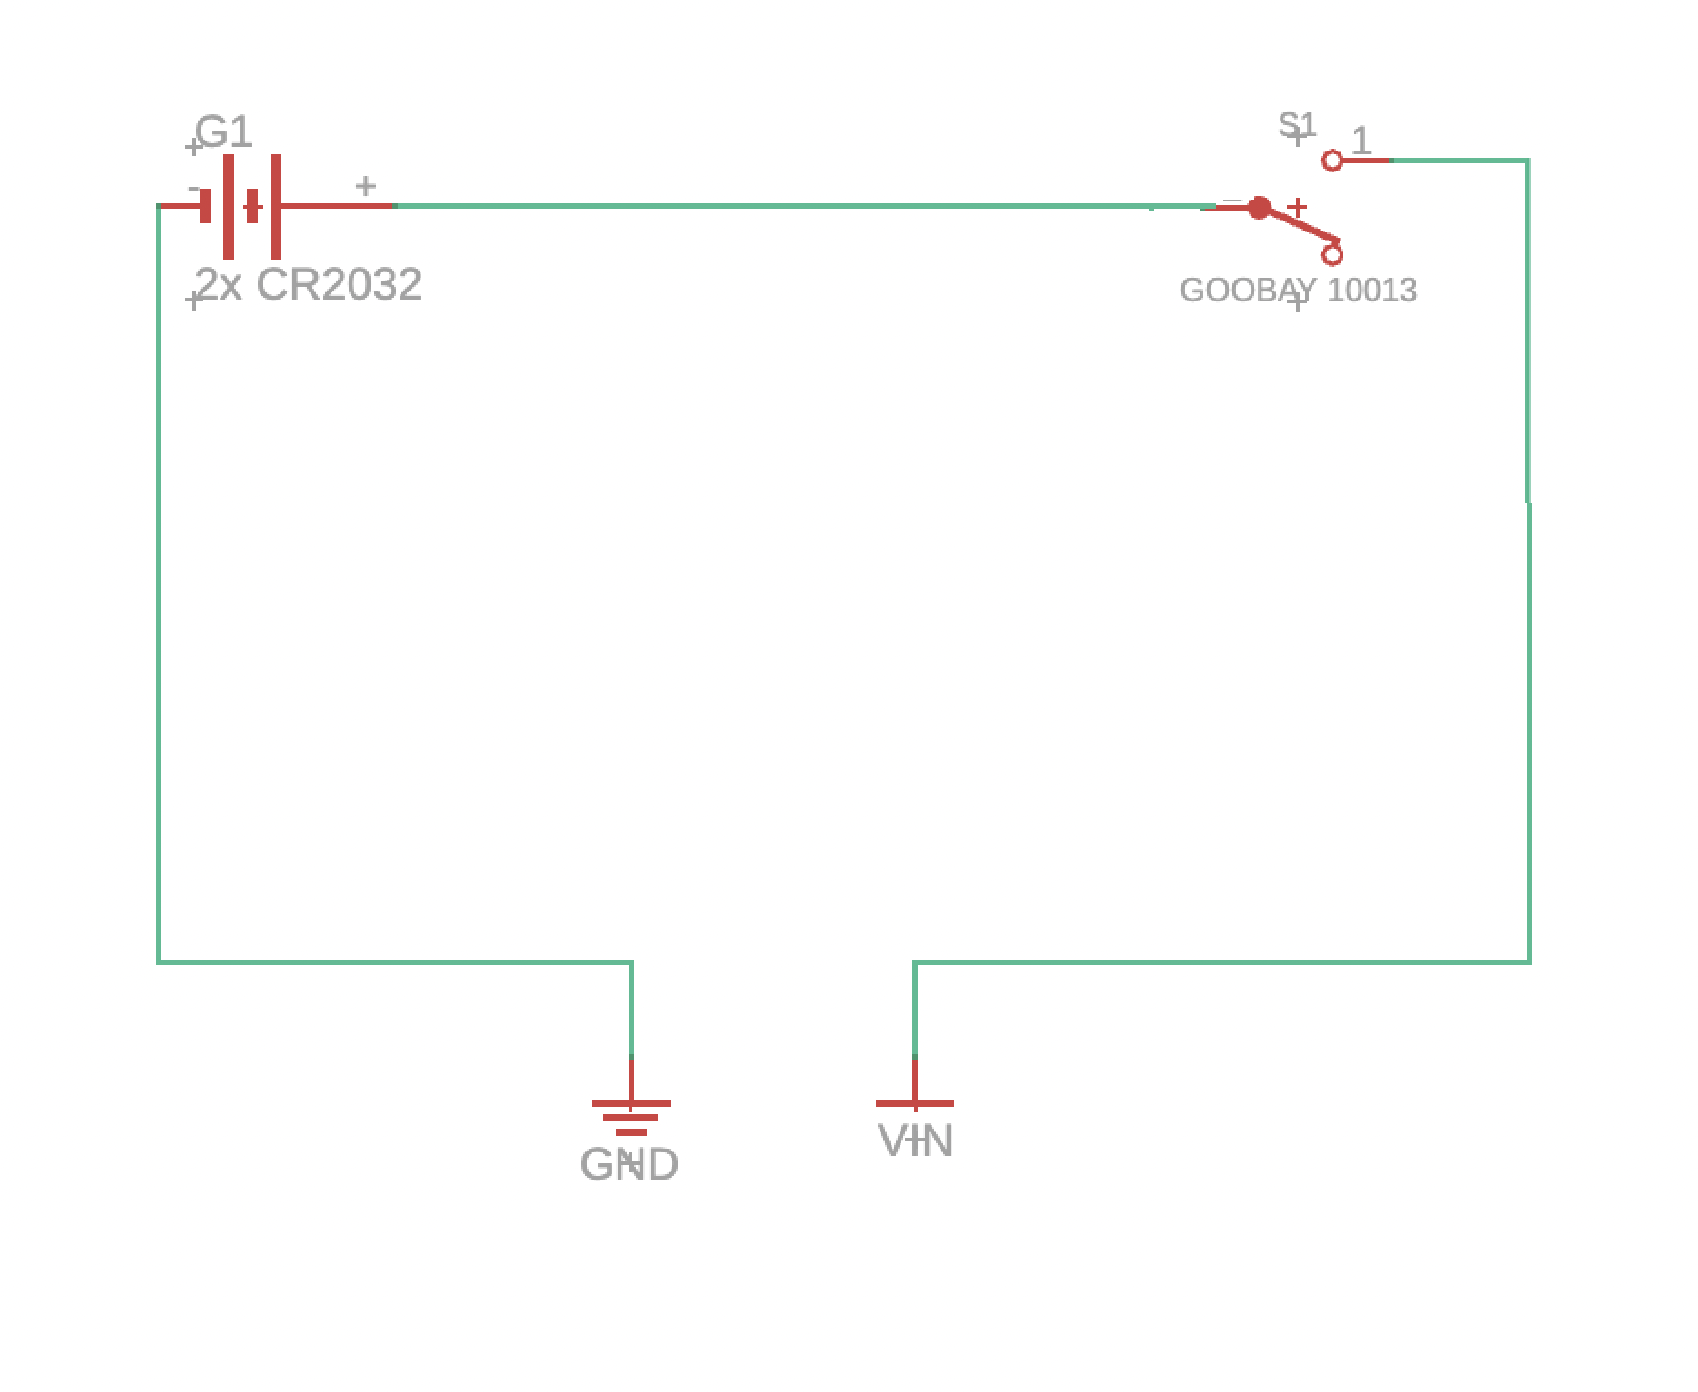
\includegraphics[width=1\textwidth]{Images/circuit} % Adjust the path and width as needed
	\caption{Battery Circuit}
	\label{fig:Battery_Circuit}
\end{figure}

\vspace{5pt} % Optional spacing
\noindent
\textbf{Component Description:}  
\vspace{5pt} % Optional spacing
\noindent



\begin{itemize}
    \item \textbf{G1:} 
    Battery pack (6V, 2x CR2032 cells), supplying power to the circuit.

    \item \textbf{S1:} 
    GOOBAY 10013 toggle switch:
    \begin{itemize}
        \item Connected to the positive terminal of the battery.
        \item Controls the power supply to the device (Arduino Nano 33 BLE Sense).
        \item Has two positions:
        \begin{itemize}
            \item \textbf{Open:} Disconnects the circuit, effectively cutting off the power supply.
            \item \textbf{Close:} Completes the circuit, enabling power to flow to the Arduino Nano 33 BLE Sense.
        \end{itemize}
    \end{itemize}

    \item \textbf{GND:} 
    Ground pin of the Arduino Nano 33 BLE Sense, connected to the negative terminal of the battery.\ref{fig:BatteryCircuitBoard}

    \item \textbf{VIN:} 
    Voltage input pin of the Arduino Nano 33 BLE Sense, where the positive terminal of the battery is connected to supply power.\ref{fig:BatteryCircuitBoard}
\end{itemize}

\begin{figure}[h]
	\centering
	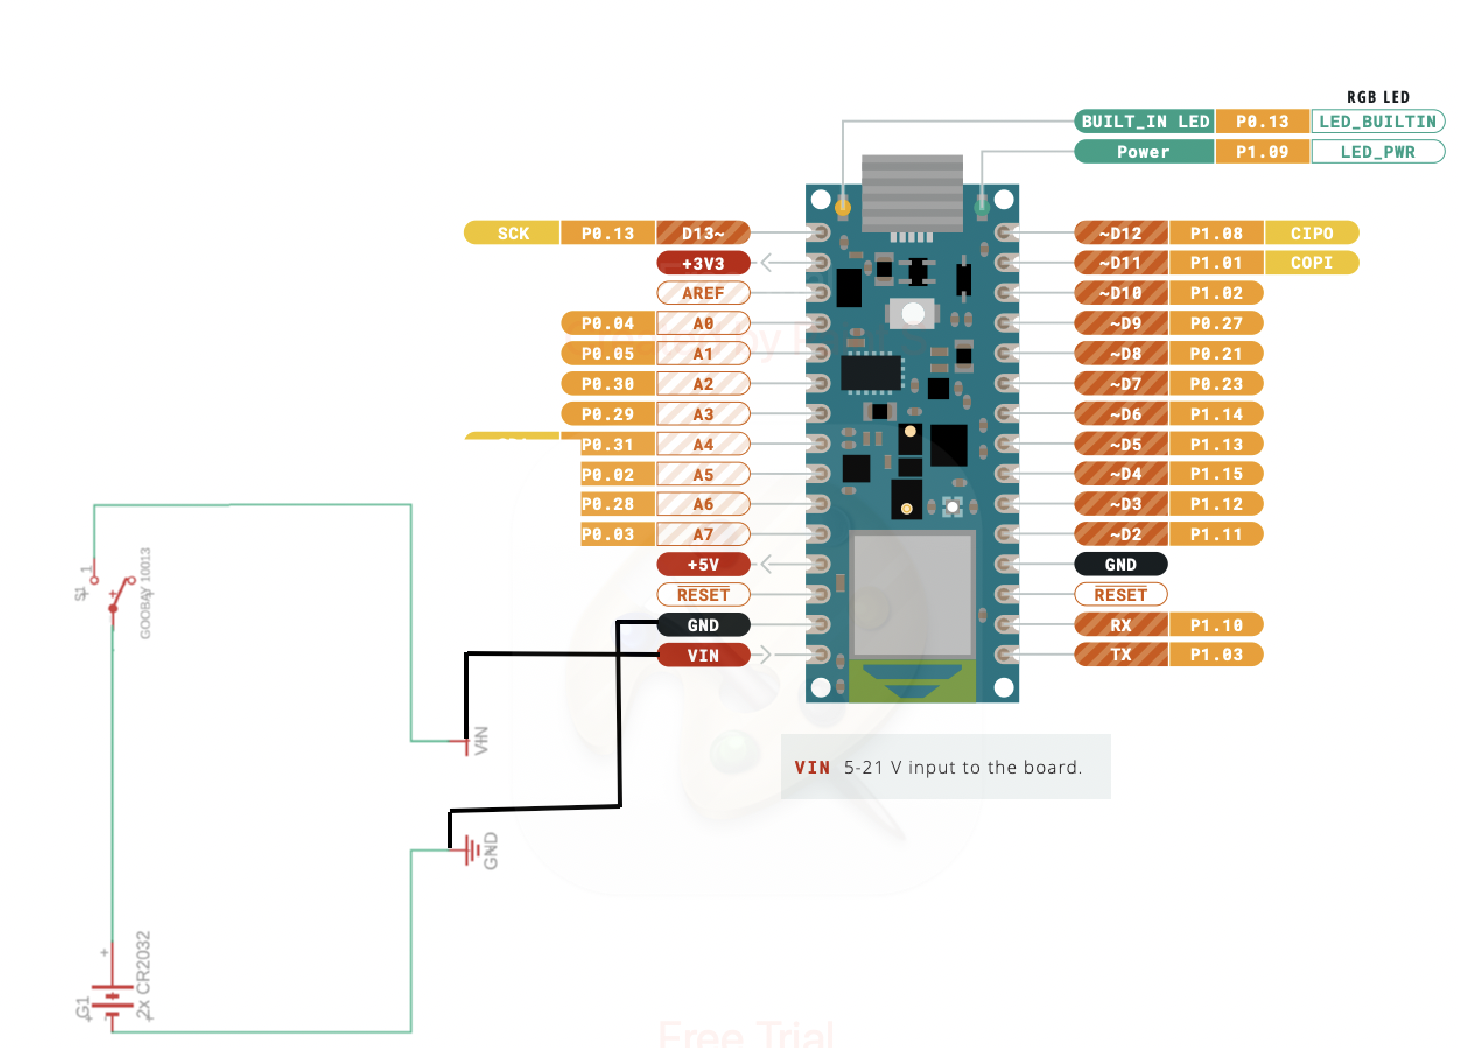
\includegraphics[width=1\textwidth]{Images/circuitboard} % Adjust the path and width as needed
	\caption{Battery Circuit and Board}
	\label{fig:BatteryCircuitBoard}
\end{figure}

\section{Battery Connected to the VIN Pin Alongside a USB Connection}

When a battery is connected to the VIN pin alongside a USB connection, the Arduino Nano 33 BLE Sense's power system ensures safe operation through diode isolation and voltage regulation.

The onboard diodes (\textbf{D2} and \textbf{D1}) play critical roles in this configuration:
\begin{itemize}
    \item If both USB and VIN are connected, the \textbf{VIN pin} takes priority, isolating the USB power supply. The diodes \textbf{D2} and \textbf{D1} prevent backflow from the VIN pin to the USB power line, protecting the USB source and board components.
    \item The voltage regulator (\textbf{MPM3610}) steps down the input voltage from VIN (4.5V–21V) or USB (5V via D2) to a stable 3.3V, ensuring safe operation of the board.
    \item If only USB is connected, power flows through \textbf{D2} to the VIN pin, enabling the MPM3610 regulator to function.
    \item If only a battery is connected to VIN, the regulator directly steps down the battery voltage to power the board.
\end{itemize}

The priority of power sources ensures that the board is safely powered, regardless of whether one or both sources are connected. The voltage regulator (\textbf{MPM3610}) consistently provides a stable 3.3V to the board under all conditions.


\begin{figure}[h]
	\centering
	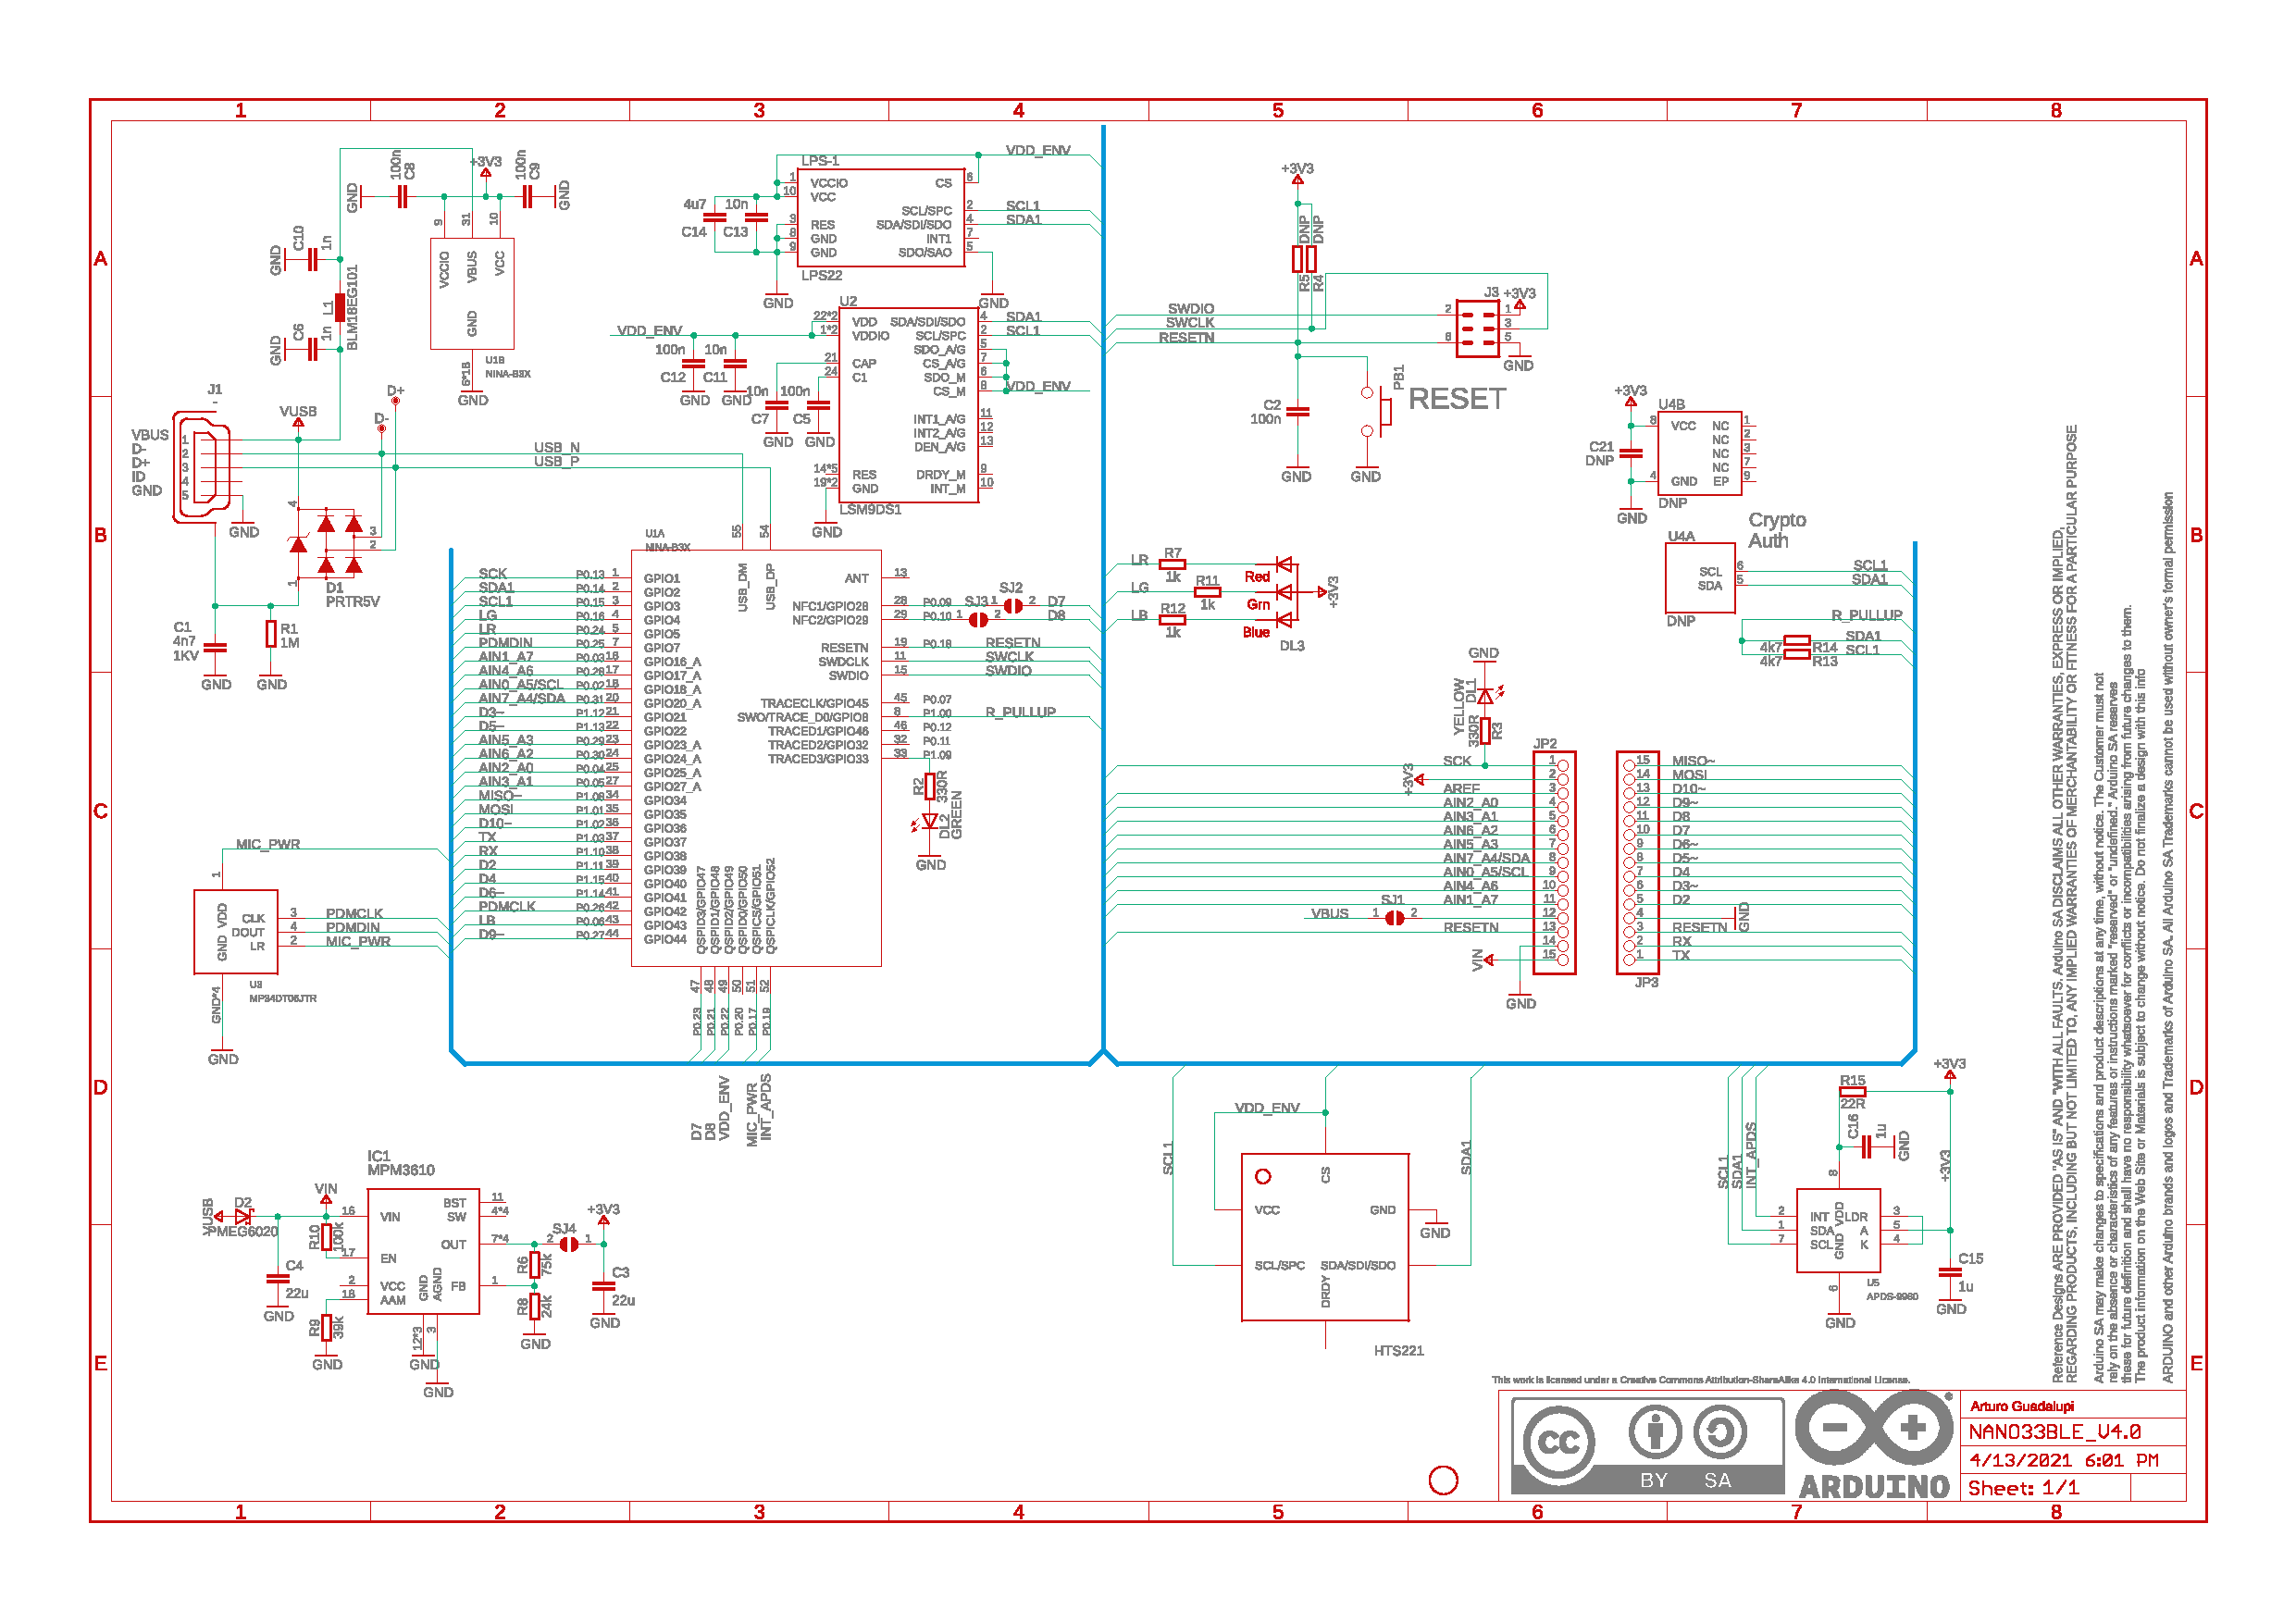
\includegraphics[width=1\textwidth]{Images/schematic} % Adjust the path and width as needed
	\caption{Schematic}
	\label{fig:Schematic}
\end{figure}


Refer to \href{https://docs.arduino.cc/resources/schematics/ABX00031-schematics.pdf}{this schematic} for a detailed diagram showing the interaction between USB, VIN, diodes \textbf{D2} and \textbf{D1}, and the voltage regulator.